\begin{figure}[h]
    \noindent\makebox[\textwidth]{
    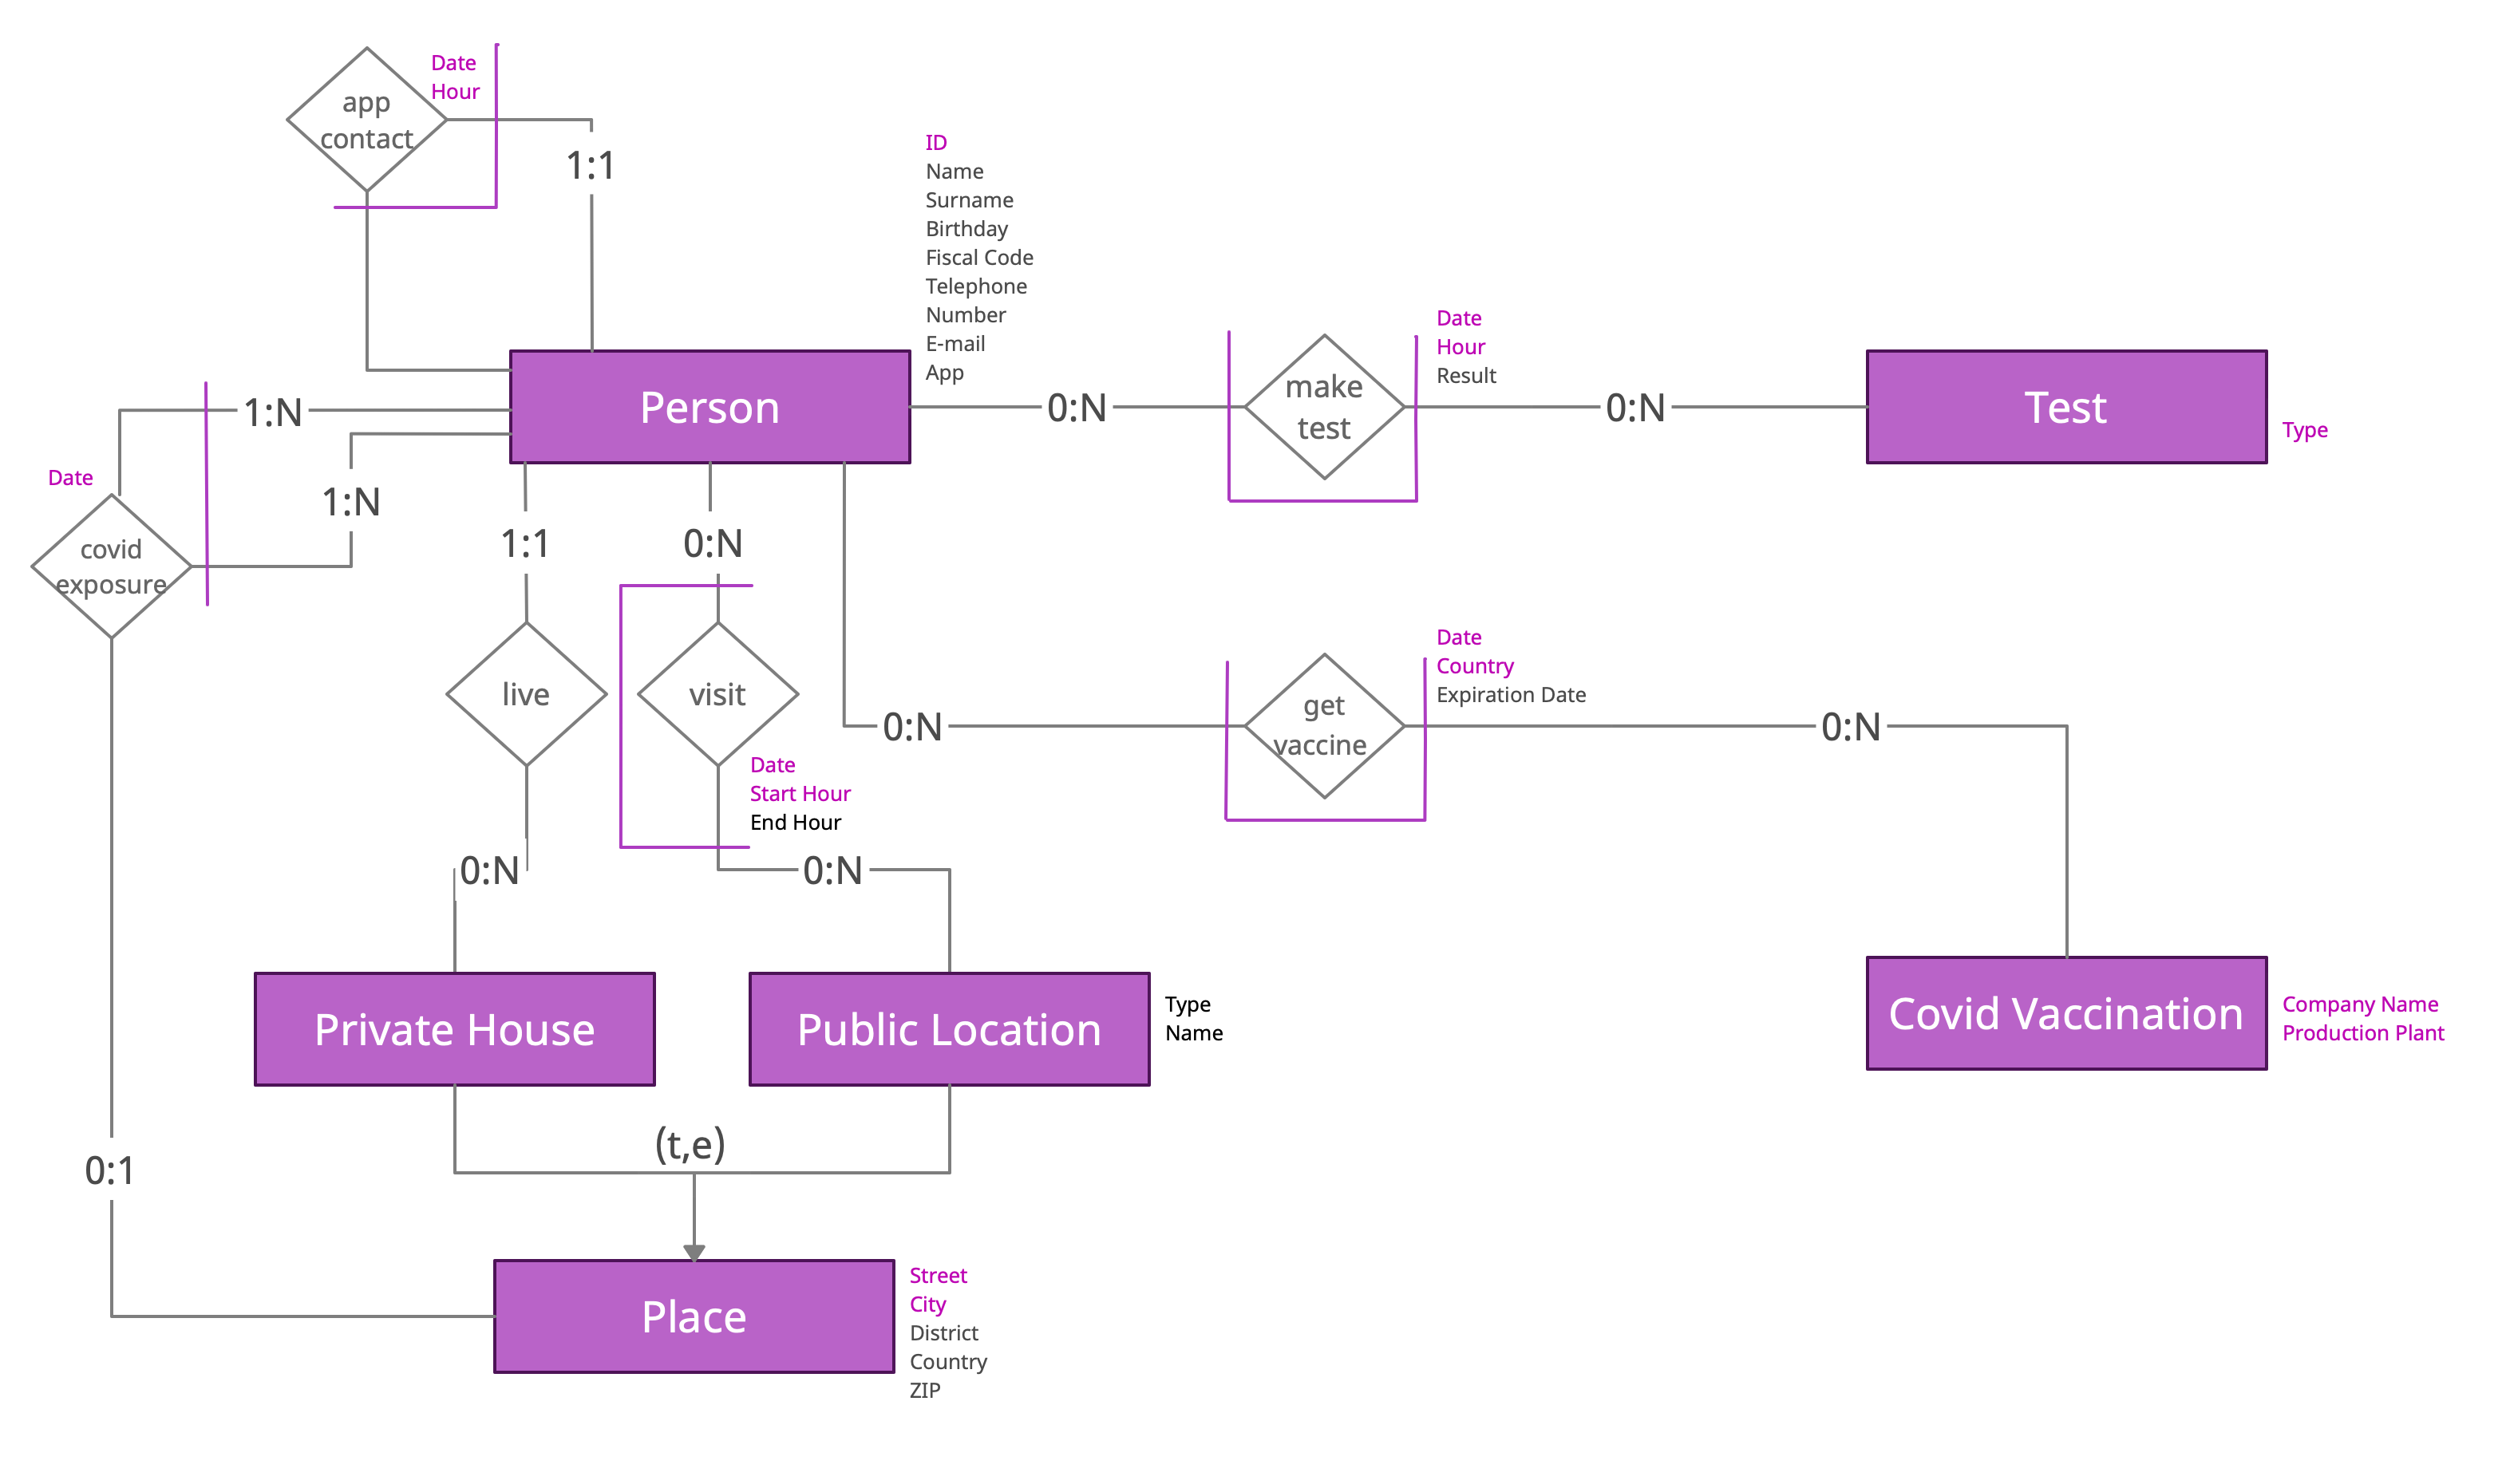
\includegraphics[width=0.8\paperwidth]{images/ImmunoPoli-ER.jpg}
    }
\caption{\textit{Entity Relationship model}}
\end{figure}

\subsection{Entities}
\begin{itemize}
    \item \textbf{Person:} man or woman identified by a unique ID. The ID is also the key for logging into the app. The property \textit{app} is a boolean attribute used to identify whether or not the person has any type of contact tracing application.
    \item \textbf{Place:} general concept of place characterized by an address.
    \item \textbf{Private house:} place that hosts either a group of flatmates or a family. The name of the house corresponds to the owner's name and surname. 
    \item \textbf{Public place:} represents indoor places accessible providing personal information for traceability purposes.
    \item \textbf{Covid Vaccination:} the COVID-19 vaccines. 
    They are identified through their company name and the production plant from where they come.
    \item \textbf{Test:} the COVID-19 tests. They are identified through their class. The distinction is between the tests that detect the viral presence through the \textit{PCR}, \textit{Molecular}, \textit{Antibody} (to check the presence of the virus antagonists) and in the end, the \textit{Rapid} ones. 
\end{itemize}

\subsection{Relationships}
\begin{itemize}
    \item The \textit{\textbf{covid exposure}} relationship represents a \emph{possible viral infection}. Once a positive test is inserted into the database, the system triggers a command\footnote{see section \ref{section: 6} for further details about the command.} to easily find all the people at risk of contagion and notify them of the possible infection. People are obliged to make a swab, and in case of a negative result after at least seven days, the relationship is deleted.
    \item The \textit{\textbf{live}} relationship binds a person with where he resides.
    \item The \textit{\textbf{visit}} relationship involves all the public places where it is more likely that personal information is collected. It serves both realism and simplicity purposes because we don't need to take care of outdoor spots.
    \item The \textit{\textbf{app contact}} relationship gathers all contacts detected by any tracking system that supports localization and applications installation, regardless of its type.
    \item The \textit{\textbf{make test}} relationship links the user with a tests he has made. It contains information such as the hour, the date and the outcome.
    \item The \textit{\textbf{get vaccine}} relationship connects the user to the vaccine he got. As well as \emph{make test}, it is characterized by the date and hour of the injection.
\end{itemize}